\documentclass[conference]{IEEEtran}
\usepackage[utf8]{inputenc}
\usepackage[T1]{fontenc}
\usepackage{cite}
\usepackage{amsmath,amssymb,amsfonts}
\usepackage{graphicx}
\usepackage{textcomp}
\usepackage{xcolor}
\usepackage{booktabs}
\usepackage{tabularx}
\usepackage{multirow}
\usepackage{url}
\usepackage{tikz}
\usetikzlibrary{arrows.meta,positioning,shapes.geometric,fit,calc}
\usepackage{hyperref}
\hypersetup{colorlinks=true,citecolor=blue,linkcolor=blue,urlcolor=blue}

\begin{document}

\title{Next-Generation Firewalls and Open-Source Adaptive Firewalls:\\A Literature Survey on ML-Augmented Network Defence}

\iffalse
\author{
\IEEEauthorblockN{Bindu N}
\IEEEauthorblockA{ENG22CY0031\\Dept.\ of CSE (Cyber Security)\\Dayananda Sagar University}
\and
\IEEEauthorblockN{Ramya D}
\IEEEauthorblockA{ENG22CY0018\\Dept.\ of CSE (Cyber Security)\\Dayananda Sagar University}
\and
\IEEEauthorblockN{Bansidharee Maji}
\IEEEauthorblockA{ENG22CY0006\\Dept.\ of CSE (Cyber Security)\\Dayananda Sagar University}
}
\fi

\maketitle

% ============================================================
\begin{abstract}
Traditional firewalls relying on static rules and port-based filtering are proving insufficient against ever-evolving digital threats. Next-Generation Firewalls (NGFWs) integrate deep packet inspection, application awareness, and intrusion prevention, but these capabilities remain confined to expensive proprietary platforms. This survey traces the evolution from packet filters to NGFWs, reviews machine learning-based intrusion detection with emphasis on Isolation Forest anomaly detection, and examines the open-source firewall ecosystem. Through a comparative analysis and systematic gap identification, we find that adaptive, behaviour-driven, ML-augmented detection is largely absent in open-source firewalls. We argue that a modular sidecar architecture pairing an open-source firewall with a lightweight ML engine represents a viable research direction for democratising adaptive network defence. Our analysis covers over 30 papers from 1987 to 2024, spanning IEEE, ACM, Springer, Elsevier, NIST, and MDPI venues.
\end{abstract}

\begin{IEEEkeywords}
Next-Generation Firewall, NGFW, Intrusion Detection, Anomaly Detection, Isolation Forest, Machine Learning, Open-Source Firewall, OPNsense
\end{IEEEkeywords}

% ============================================================
\section{Introduction}
\label{sec:intro}

The cybersecurity landscape has been shifting at an alarming pace. Traditional firewalls, operating by matching packets against static rule sets of IP addresses, port numbers, and protocol identifiers, are fundamentally limited in detecting application-layer attacks, zero-day exploits, and behavioural anomalies \cite{neupane2018ngfw, liang2022evolution}. The industry responded with Next-Generation Firewalls (NGFWs), combining standard firewall capabilities with IDS/IPS, deep packet inspection (DPI), and application awareness \cite{heino2022endpoint}. However, the commercial NGFW market, dominated by Palo Alto Networks, Fortinet, Check Point, and Cisco, keeps advanced capabilities inaccessible to smaller organisations and researchers.

Open-source firewalls such as OPNsense and pfSense have matured for packet filtering, NAT, VPN, and signature-based IDS through Suricata integration \cite{kiratsata2022behaviour}, but they lack native support for adaptive, behaviour-based anomaly detection. This gap represents a meaningful research opportunity that the academic community has only recently begun to explore.

This survey provides a comprehensive review of firewall evolution, NGFW architecture, ML-based intrusion detection, and the open-source ecosystem, establishing the motivation for investigating ML-augmented open-source firewall architectures. Section~\ref{sec:background} covers background, related work, and the evolution from packet filters to NGFWs. Section~\ref{sec:architecture} examines modern NGFW architecture. Section~\ref{sec:comparative} presents a comparative analysis. Section~\ref{sec:ml} reviews ML approaches. Sections~\ref{sec:gap}--\ref{sec:motivation} identify gaps and discuss research directions.

% ============================================================
\section{Background and Related Work}
\label{sec:background}

This section provides both a structured overview of the key literature underpinning this survey (Table~\ref{tab:lit_survey}) and a concise account of how firewall technology evolved from simple packet filters to the NGFW platforms available today. The literature spans firewall architecture \cite{neupane2018ngfw, liang2022evolution, scarfone2009nist}, intrusion detection theory \cite{denning1987ids, khraisat2019ids}, anomaly detection methodology \cite{chandola2009anomaly, liu2008isolation, tao2018parallel}, and ML-based IDS design \cite{ahmad2021nids, dini2023overview}. Together, these works establish that while ML-based anomaly detection has been proven effective in controlled settings, its integration into open-source firewalls remains an unexplored intersection that this survey aims to characterise.

\begin{table*}[!t]
\centering
\caption{Summary of Key Literature Informing This Survey}
\label{tab:lit_survey}
\renewcommand{\arraystretch}{1.3}
\scriptsize
\begin{tabularx}{\textwidth}{p{2.6cm} p{1.5cm} X p{2.2cm} X}
\toprule
\textbf{Paper Title} & \textbf{Authors \& Year} & \textbf{Key Contributions} & \textbf{Methodology} & \textbf{Relevance to This Work} \\
\midrule
An Intrusion-Detection Model & Denning, 1987 \cite{denning1987ids} & \textbullet~Founded anomaly-based intrusion monitoring via statistical profiles on audit trails & Statistical audit-trail profiling & \textbullet~Theoretical basis for behaviour-based anomaly detection \\
\midrule
Next Generation Firewall for Network Security: A Survey & Neupane et al., 2018 \cite{neupane2018ngfw} & \textbullet~Comprehensive NGFW taxonomy tracing evolution from packet filters to NGFWs & Systematic literature review & \textbullet~Core framework for the firewall evolution analysis \\
\midrule
Evolution of Firewalls: Toward Securer Network Using NGFW & Liang \& Kim, 2022 \cite{liang2022evolution} & \textbullet~Analysed single-pass NGFW architecture and UTM-to-NGFW transition & Case study of commercial NGFW & \textbullet~Informs pipeline design and NGFW advantage discussion \\
\midrule
Isolation Forest & Liu et al., 2008 \cite{liu2008isolation} & \textbullet~Proposed linear-time unsupervised anomaly detection via random recursive partitioning & Ensemble of isolation trees with path-length scoring & \textbullet~Core algorithm adopted for network anomaly detection \\
\midrule
Anomaly Detection: A Survey & Chandola et al., 2009 \cite{chandola2009anomaly} & \textbullet~Comprehensive taxonomy of anomaly types and detection approaches across domains & Cross-domain systematic review & \textbullet~Theoretical foundation for defining network anomalies \\
\midrule
Network Intrusion Detection System: A Systematic Study & Ahmad et al., 2021 \cite{ahmad2021nids} & \textbullet~Compared ML and DL for NIDS; found traditional ML competitive for real-time detection & Systematic review of ML/DL classifiers & \textbullet~Justifies lightweight ML over deep learning choice \\
\midrule
Survey of Intrusion Detection Systems & Khraisat et al., 2019 \cite{khraisat2019ids} & \textbullet~Analysed IDS operational overhead and false positive impact on deployment viability & Survey of IDS techniques, datasets, challenges & \textbullet~Informs discussion of IDS limitations and FP challenges \\
\midrule
Parallel Isolation Forest for Network Traffic Anomaly Detection & Tao et al., 2018 \cite{tao2018parallel} & \textbullet~Validated Isolation Forest on real-world network traffic at scale & Parallel IF on Apache Spark with flow features & \textbullet~Confirms IF effectiveness with statistical flow features \\
\midrule
Guidelines on Firewalls and Firewall Policy (NIST SP~800-41) & Scarfone \& Hoffman, 2009 \cite{scarfone2009nist} & \textbullet~Authoritative firewall classification and deployment policy framework & NIST technical guideline & \textbullet~Provides the firewall taxonomy used in this survey \\
\midrule
Overview on IDS Design Exploiting ML for Cybersecurity & Dini et al., 2023 \cite{dini2023overview} & \textbullet~Identified gap between academic ML accuracy and practical production deployment & Review of ML-based IDS design approaches & \textbullet~Motivates the sidecar integration architecture \\
\bottomrule
\end{tabularx}
\end{table*}

\subsection{Evolution of Firewall Technology}

The history of network firewalls begins with the Morris Worm of November 1988, which brought roughly 10\% of the Internet's connected machines to a crawl and prompted DARPA to fund the CERT Coordination Centre \cite{ingham2002history}. First-generation \textit{packet filters} appeared between 1988 and 1990, notably Mogul's \texttt{screend} daemon at DEC and early circuit-level gateways at AT\&T Bell Labs \cite{cheswick1994firewalls}. These systems made binary accept/reject decisions based solely on Layer~3/4 headers: computationally efficient but stateless and blind above Layer~4 \cite{mukkamala2020survey}. Application-level gateways (proxies) followed in 1991--92, offering Layer~7 inspection at the cost of latency and scalability \cite{george2021brief}. The pivotal advance was \textit{stateful inspection} in 1994 with Check Point's FireWall-1, which maintained connection state tables and became the architectural foundation for all modern firewalls \cite{scarfone2009nist}. Table~\ref{tab:timeline} summarises these and subsequent milestones.

\begin{table}[!t]
\centering
\caption{Key Milestones in Firewall History}
\label{tab:timeline}
\renewcommand{\arraystretch}{1.15}
\small
\begin{tabularx}{\columnwidth}{c|X}
\toprule
\textbf{Year} & \textbf{Milestone} \\
\midrule
1988 & Morris Worm; CERT/CC founded \\
1989 & Mogul's \texttt{screend} packet filter (DEC) \\
1991 & Ranum's DEC SEAL proxy firewall \\
1993 & TIS Firewall Toolkit (FWTK) released \\
1994 & Check Point FireWall-1 (stateful inspection) \\
1998 & Snort IDS released by Roesch \cite{roesch1999snort} \\
2004 & Gartner coins ``UTM'' category \\
2009 & Gartner defines ``NGFW'' category \\
2015 & OPNsense forked from pfSense \\
2020s & ML-augmented firewalls emerge in research \\
\bottomrule
\end{tabularx}
\end{table}

The mid-2000s saw the emergence of \textit{Unified Threat Management} (UTM) devices, which bundled firewall, antivirus, VPN, and basic IDS into a single appliance. UTM prioritised breadth of coverage but often suffered performance bottlenecks when all features were enabled simultaneously \cite{neupane2018ngfw}. The \textit{Next-Generation Firewall} (NGFW), formalised by Gartner in 2009, shifted perimeter security from ``block known threats'' towards ``understand and decide'' \cite{liang2022evolution}. NGFWs integrate application identification along with full-stack visibility, and threat intelligence into a single-pass processing pipeline which significantly reduces latency compared to chained inspection engines \cite{heino2022endpoint}. Singh and Singh \cite{singh2024comparative} found that NGFWs provide substantially better protection against application-layer and encrypted threats although the performance-security tradeoff remains a concern for resource-constrained deployments. The boundary between UTM and NGFW has been blurred; modern NGFWs which includes URL filtering, sandboxing, and DNS security, but the key differentiator remains depth of inspection versus breadth of features \cite{neupane2018ngfw}. Fig.~\ref{fig:evolution} illustrates this evolutionary lineage.

%insert evolution image here

\begin{figure*}[!htbp]
    \centering
    
\includegraphics[width=\textwidth]{firewall evolution.jpg}
    \caption{Evolutionary flow of network defence systems\cite{neupane2018ngfw, liang2022evolution}.}
    \label{fig:evolution}
\end{figure*}




% ============================================================
\section{Architecture of Modern NGFW}
\label{sec:architecture}

A modern NGFW distinguishes itself from the rest through several tightly integrated components. \textit{Deep Packet Inspection} (DPI) examines full packet payloads which enables protocol identification regardless of port and content-based filtering; Song et al.\ \cite{song2020dpi} demonstrated that software-based DPI achieves real-time anomaly detection without specialised hardware, though encrypted traffic (TLS~1.3, QUIC) poses challenges \cite{heino2022endpoint}. \textit{Application Control} identifies thousands of applications through protocol decoding and heuristic matching even on non-standard ports \cite{liang2022evolution}; Islam et al.\ \cite{islam2023analysis} found that properly configured application policies significantly reduce the attack surface. \textit{Integrated IDS/IPS} operates within the same inspection pipeline, leveraging application context for more accurate detection \cite{neupane2018ngfw}, while \textit{Threat Intelligence} provides real-time updates on malicious indicators from cloud services \cite{lamdakkar2024modern}. Table~\ref{tab:ngfw_components} maps these components to OSI layers.

\begin{table}[!t]
\centering
\caption{NGFW Architectural Components}
\label{tab:ngfw_components}
\renewcommand{\arraystretch}{1.2}
\begin{tabularx}{\columnwidth}{l|l|X}
\toprule
\textbf{Component} & \textbf{Layer} & \textbf{Function} \\
\midrule
Packet Filter & L3/L4 & ACL-based accept/deny \\
Stateful Engine & L4 & Connection tracking \\
DPI Engine & L4--L7 & Payload analysis \\
App-ID & L7 & Application identification \\
IPS Module & L3--L7 & Signature \& anomaly rules \\
Threat Intel & L3--L7 & IoC matching \\
SSL/TLS Proxy & L5 & Encrypted traffic inspection \\
\bottomrule
\end{tabularx}
\end{table}

% ============================================================
\section{Comparative Analysis of Defence Systems}
\label{sec:comparative}

The network defence mechanisms vary in terms of important qualitative characteristics. Conventional firewalls are deterministic in enforcing a set of policies but are completely unadaptable since the rules are fixed unless manually changed \cite{scarfone2009nist}. IDS is based on the intrusion detection model developed by Denning in 1987 \cite{denning1987ids}, which introduced the concept of observation-based monitoring. IDS is structurally limited in terms of alert fatigue, (Liao et al.\ in \cite{liao2013ids}showed that IDS generates thousands of daily alerts, which are usually false positives and passivity, the fact that IDS does not enforce the rules. IPS solves the passivity problem but introduces the problem of false positives causing legitimate data to be dropped instead of flagged \cite{khraisat2019ids}. IDS was popularized by the development of the Snort \cite{roesch1999snort} and Bro/Zeek \cite{paxson1999bro} systems but was limited by the noise and passivity problem.

The UTM solves the noise problem by bundling multiple engines but is plagued by the problem of monolithism and degradation in performance when the full features are enabled \cite{neupane2018ngfw}. NGFW solves the contextual intelligence problem through a single-pass approach \cite{liang2022evolution},  but the vendor lock-in problem is a major concern. There is an interesting trend in the evolution of defence mechanisms, the assimilation of features from other technologies. Firewalls assimilated connection tracking, proxy servers, and then antivirus, VPN, IDS (UTM), application identification and threat intelligence (NGFW), and are now assimilating machine learning and behavioral analysis from the NGFW. The assimilation trend is a result of the architectural requirement for a single point of enforcement \cite{neupane2018ngfw}.

The human-in-the-loop aspect of adapting the defence mechanism in response to changing network conditions is still a manual task and is the biggest weakness in the entire framework. The human-in-the-loop problem is a result of the inability of the defence mechanism to apply machine learning or statistical inference techniques. This is a recurring theme in the discussion of the limitations of open-source defence mechanisms \cite{ahmad2021nids, dini2023overview}. Table~\ref{tab:comparative} summarizes the characteristics of the seven system classes.

\begin{table*}[!t]
\centering
\caption{Comparative Analysis of Packet-Level Defence Systems}
\label{tab:comparative}
\renewcommand{\arraystretch}{1.15}
\small
\begin{tabularx}{\textwidth}{l|c|c|c|c|c|c}
\toprule
\textbf{System} & \textbf{Inspect.\ Layer} & \textbf{Detection Type} & \textbf{Prevention} & \textbf{ML Integr.} & \textbf{Adaptability} & \textbf{Open-Source} \\
\midrule
Stateless Firewall    & L3/L4 headers    & Rule-based         & Inline drop  & None      & None       & Yes (iptables) \\
Stateful Firewall     & L3/L4 + state    & Rule + state       & Inline drop  & None      & None       & Yes (pf, nftables) \\
IDS                   & L3--L7 payload   & Signature + anom.  & Alert only   & Rare      & Low        & Yes (Snort, Suricata) \\
IPS                   & L3--L7 payload   & Signature + anom.  & Inline drop  & Rare      & Low        & Yes (Suricata) \\
UTM                   & L3--L7 mixed     & Multi-engine       & Inline       & None      & Low        & Partial (Endian) \\
NGFW                  & L3--L7 full      & Contextual + sig   & Inline       & Emerging  & Moderate   & Limited \\
AI-Augmented FW       & L3--L7 + behav.  & Learned baseline   & Automated    & Core      & High       & Underexplored \\
\bottomrule
\end{tabularx}
\end{table*}

% ============================================================
\section{Machine Learning in Network Security}
\label{sec:ml}

\subsection{ML-Based Intrusion Detection}

Ahmad et al.\ \cite{ahmad2021nids} systematically reviewed ML and deep learning for NIDS, finding that while deep learning achieves higher accuracy on benchmarks, traditional ML remains competitive in real-time scenarios due to lower computational requirements. Liu and Lang \cite{liu2019mlids} highlighted that unsupervised methods are particularly relevant for novel attack detection where labeled data is unavailable. Da Costa et al.\ \cite{dacosta2019iot} argued that resource constraints favour lightweight algorithms like Isolation Forest over deep learning.

Most published IDS research uses supervised learning on benchmark datasets \cite{zhang2022comparative}. Table~\ref{tab:datasets} summarises widely used benchmarks. Zhang et al.\ \cite{zhang2022comparative} found that ensemble approaches (Random Forest, XGBoost) outperform individual classifiers but exhibit poor cross-dataset generalisation, suggesting overfitting to dataset-specific artefacts. Unsupervised approaches, grounded in Chandola et al.'s \cite{chandola2009anomaly} theoretical framework, detect anomalies as deviations from learned normal behaviour without requiring labeled data.

\begin{table}[!t]
\centering
\caption{Widely Used IDS Benchmark Datasets}
\label{tab:datasets}
\renewcommand{\arraystretch}{1.15}
\small
\begin{tabularx}{\columnwidth}{l|c|c|X}
\toprule
\textbf{Dataset} & \textbf{Year} & \textbf{Records} & \textbf{Attack Types} \\
\midrule
KDD Cup 99   & 1999 & $\sim$5M   & DoS, R2L, U2R, Probe \\
NSL-KDD      & 2009 & $\sim$150K & Cleaned KDD subset \\
UNSW-NB15    & 2015 & $\sim$2.5M & Fuzzers, Backdoor, DoS \\
CICIDS2017   & 2017 & $\sim$2.8M & DDoS, Botnet, Infiltration \\
CSE-CIC-IDS  & 2018 & $\sim$1M   & Updated attack profiles \\
\bottomrule
\end{tabularx}
\end{table}

He et al.\ \cite{he2023adversarial} raised the concern that ML-based detection systems are themselves vulnerable to adversarial attacks, a valid consideration for production systems, though beyond the scope of initial feasibility studies. Vartouni et al.\ \cite{vartouni2019leveraging} demonstrated that deep neural networks can effectively distinguish legitimate from malicious traffic at L7, while Dini et al.\ \cite{dini2023overview} identified feature engineering, dataset quality, and infrastructure integration as the main barriers to deploying ML-based detection in practice.

\subsection{Isolation Forest for Anomaly Detection}

The Isolation Forest algorithm \cite{liu2008isolation} is among the most practical unsupervised methods for network anomaly detection. Its core insight is that anomalies, being ``few and different,'' are easier to isolate through random partitioning. Given $n$ observations, an ensemble of $t$ isolation trees (iTrees) recursively partitions data by random feature splits. The path length $h(\mathbf{x})$ from root to terminating node yields the anomaly score:
\begin{equation}
\label{eq:iforest_score}
s(\mathbf{x}, n) = 2^{-\frac{E[h(\mathbf{x})]}{c(n)}}
\end{equation}
where $E[h(\mathbf{x})]$ is the average path length over all $t$ trees, and $c(n)$ is the average unsuccessful BST search path length serving as normalisation:
\begin{equation}
\label{eq:cn}
c(n) = 2H(n-1) - \frac{2(n-1)}{n}
\end{equation}
with $H(i) = \ln(i) + \gamma$ (harmonic number, $\gamma \approx 0.5772$). Scores near~1 indicate anomalies (short paths); scores near~0.5 indicate normal instances \cite{liu2008isolation}.

Al Farizi et al.\ \cite{alfarizi2021isolation} reviewed over 100 Isolation Forest applications and found consistently competitive performance with significantly lower computational cost than other unsupervised methods. Tao et al.\ \cite{tao2018parallel} confirmed that Isolation Forest detects volumetric, protocol, and behavioural anomalies with high precision at scale on real-world traffic. Cheng et al.\ \cite{cheng2019outlier} showed it is substantially faster and more memory-efficient than Local Outlier Factor (LOF), making it preferred for real-time applications.

\subsection{Feature Engineering}

Flow-level statistical features, packets per second, byte rates, inter-arrival times, protocol ratios, TCP flag distributions, operate on packet metadata rather than payload, making them applicable even to encrypted traffic \cite{tao2018parallel, ahmad2021nids}. Sultana et al.\ \cite{sultana2019sdn} confirmed that such features are well-suited for flow-based detection architectures. These features can reveal volumetric, protocol, and behavioural anomalies without any payload access, which is increasingly important as TLS~1.3 and QUIC adoption grows.

% ============================================================
\section{Open-Source Firewall Ecosystem}
\label{sec:opensource}

OPNsense, forked from pfSense in 2015, is built on HardenedBSD with a modern web interface and plugin architecture \cite{che2023opnsense}. Kiratsata et al.\ \cite{kiratsata2022behaviour} found comparable packet filtering performance between pfSense and OPNsense, with OPNsense offering more frequent security patches. Olivera-Ruiz et al.\ \cite{olivera2024opensource} benchmarked multiple platforms and found OPNsense and pfSense outperformed IPFire and Endian in throughput and packet loss.

Both platforms support Suricata for signature-based IDS/IPS, but Suricata's detection is fundamentally rule-based, it does not learn or adapt to the network environment \cite{dini2023overview}. None of the major open-source platforms offer native ML-based anomaly detection. This observation is consistent with Mohile's \cite{mohile2023ngfw} finding that adaptive, context-driven threat prevention remains a commercial-vendor feature. The combination of OPNsense's mature packet filtering, REST API support, and plugin architecture makes it a strong candidate for external ML augmentation.

% ============================================================
\section{Gap Analysis}
\label{sec:gap}

Based on our literature review, we identify five gaps that collectively motivate the research direction.

\textbf{Gap~1: Static vs.\ Adaptive Detection.} Open-source firewalls rely exclusively on signature-based and rule-based detection, which are fundamentally unable to detect zero-day attacks or behavioural anomalies. Commercial NGFWs address this with proprietary ML engines and cloud analytics, but no equivalent exists in the open-source space \cite{liu2019mlids, ahmad2021nids}.

\textbf{Gap~2: Absent Closed-Loop Enforcement.} Even where anomaly detection exists (e.g., Suricata alerts), response is manual, an administrator reviews alerts and decides on action. Automated feedback loops where detection triggers enforcement are absent in standard open-source deployments \cite{psychogyios2024ddos}.

\textbf{Gap~3: Dataset Relevance.} Most academic IDS research uses benchmark datasets that may not represent the traffic patterns of a specific deployment. There is limited work on generating environment-specific datasets from actual firewall logs for training localised anomaly detectors \cite{zhang2022comparative}.

\textbf{Gap~4: Integration Architecture.} Few papers demonstrate end-to-end integration from feature extraction through inference to automated firewall rule modification. The ``model to enforcement'' pathway is rarely shown as a working pipeline \cite{dini2023overview}.

\textbf{Gap~5: Signature Dependency.} The window between exploit emergence and signature availability ranges from hours to weeks \cite{khraisat2019ids}. For targeted attacks with custom tools, signatures may never be created, a fundamental limitation unsolvable within the signature paradigm \cite{liu2019mlids}.

Table~\ref{tab:gap} summarises the capability distribution across firewall types, highlighting where an ML-augmented approach would be positioned.

\begin{table}[!t]
\centering
\caption{Capability Comparison across Firewall Types}
\label{tab:gap}
\renewcommand{\arraystretch}{1.15}
\begin{tabularx}{\columnwidth}{X|c|c|c|c}
\toprule
\textbf{Capability} & \textbf{Trad.} & \textbf{UTM} & \textbf{NGFW} & \textbf{ML-Aug.} \\
\midrule
Packet Filtering & \checkmark & \checkmark & \checkmark & \checkmark \\
Stateful Inspection &, & \checkmark & \checkmark & \checkmark \\
Signature IDS/IPS &, & \checkmark & \checkmark & \checkmark \\
DPI &, & Partial & \checkmark &, \\
Application Control &, &, & \checkmark &, \\
ML Anomaly Detection &, &, & Partial & \checkmark \\
Automated Response &, &, & Partial & \checkmark \\
Open Source &, & Partial &, & \checkmark \\
\bottomrule
\end{tabularx}
\end{table}

% ============================================================
\section{Research Directions and Motivation}
\label{sec:motivation}

\subsection{The Sidecar Architecture}

Rather than modifying an open-source firewall's codebase, which would create maintenance and compatibility issues, a sidecar architecture decouples the ML engine from the firewall. The firewall remains the inline enforcement point while a companion ML engine on a separate host consumes syslog telemetry, performs feature extraction and inference, and communicates back through the firewall's REST API \cite{lamdakkar2024modern}. This allows each component to be developed, tested, and updated independently. Fig.~\ref{fig:sidecar} illustrates this pattern.


\begin{figure}
    \centering
    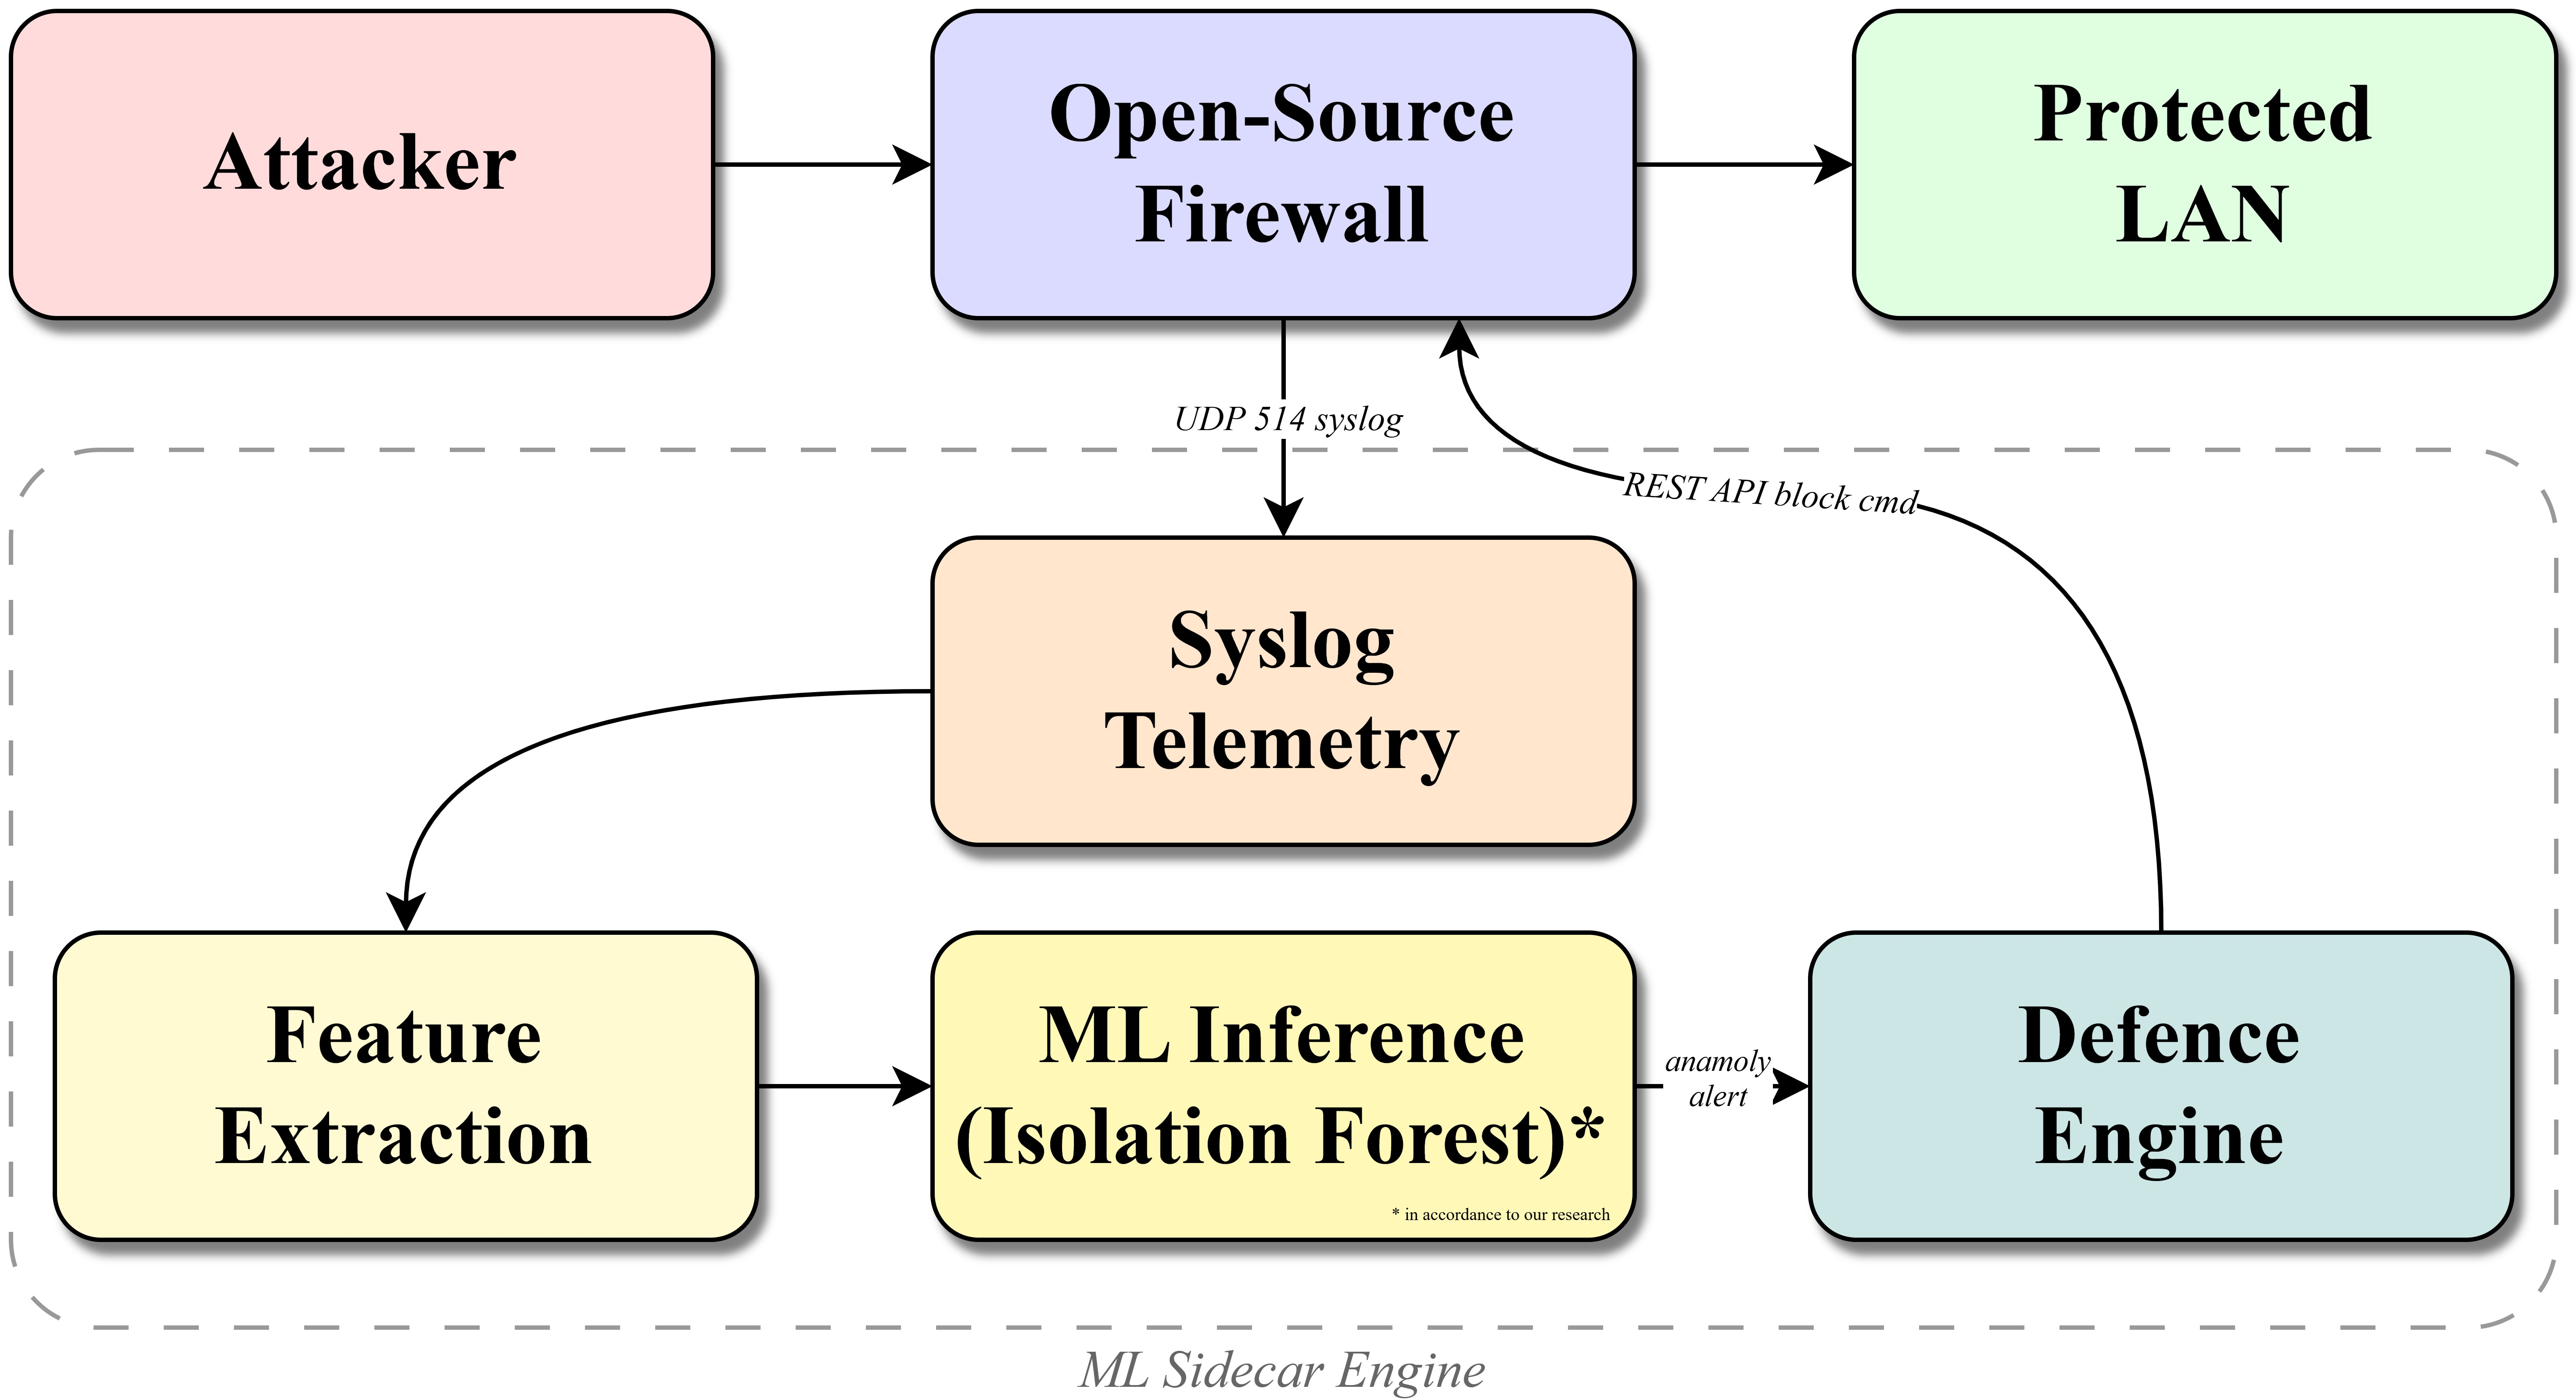
\includegraphics[width=1\linewidth]{ngfw architecture.jpg}
    \caption{Sidecar architecture for ML-augmented open-source firewall. The firewall handles inline enforcement; the sidecar consumes syslog, extracts features, runs inference, and issues block commands via REST API.}
    \label{fig:sidecar}
\end{figure}



\subsection{The Case for Isolation Forest}

Among available ML methods, Isolation Forest \cite{liu2008isolation} is attractive for this domain because it is (i)~unsupervised, no labeled attack data is needed \cite{liu2008isolation}; (ii)~computationally efficient, $O(t \cdot \psi \cdot \log \psi)$ training, $O(t \cdot \log \psi)$ inference \cite{alfarizi2021isolation}; (iii)~proven on network data \cite{tao2018parallel, cheng2019outlier}; and (iv)~available in scikit-learn without GPU dependency. Its limitations, assuming globally isolated anomalies and sensitivity to hyperparameters, warrant empirical evaluation.

\subsection{Research Opportunity}

While individual components exist (open-source firewall, Isolation Forest, syslog parsing, REST API automation), their combination into a working end-to-end pipeline has not been convincingly demonstrated. The research lies in the integration: investigating whether an open-source firewall can be augmented with an ML detection-and-response loop using entirely open tools, and evaluating practical performance, accuracy, and reliability. Flow-level statistical features derived from packet metadata are applicable regardless of encryption status and can detect L2/L3/L4 anomalies \cite{tao2018parallel, sultana2019sdn}, making this approach complementary to existing signature-based defences.

% ============================================================
\section{Conclusion}
\label{sec:conclusion}

This survey has traced firewall evolution from 1980s packet filters through stateful inspection, UTM, and modern NGFW platforms, reviewing over 30 papers spanning firewall architecture, intrusion detection, Isolation Forest anomaly detection, and open-source ecosystems. The key finding is that while commercial NGFWs increasingly integrate ML and adaptive security, the open-source ecosystem remains rooted in rule-based and signature-based paradigms. The five gaps identified, static detection, absent closed-loop enforcement, dataset irrelevance, poor integration architecture, and signature dependency, collectively point toward a research direction that is technically challenging and practically relevant. Future work should include empirical evaluation against benchmark attack datasets, investigation of online learning for model adaptation, extension to Layer~7 detection using HTTP and DNS analysis, and formal false positive rate assessment under realistic traffic conditions.

% ============================================================
\bibliographystyle{IEEEtran}
\bibliography{references}

\end{document}
